\documentclass[plainsections,  24pt]{sciposter} % 36pt no ppt eh 24pt
\usepackage[english]{babel}
\usepackage{xcolor,eso-pic,graphicx,wallpaper}
\usepackage{fix-cm} % Huge
\usepackage{amsfonts,wrapfig} %simbolos matematicos
\usepackage{amssymb,amsmath,amsthm } %simbolos matematicos
\usepackage{textcomp}
\usepackage{psfrag, color,ifpdf,multicol,xspace}
\usepackage[utf8]{inputenc}

%\renewcommand{\sfdefault}{verdana}
%\usepackage{verbatim}
\usepackage{graphicx}%
\usepackage{color}
%\usepackage[small,bf]{caption}

%\usepackage{gtamacverdana}
%\usepackage{verdana}

\providecommand{\U}[1]{\protect\rule{.1in}{.1in}}
%EndMSIPreambleData
\setcounter{tocdepth}{4}

\renewenvironment{proof}[1][Demonstração:]{\noindent\textbf{#1} }{\hfill   \rule{0.5em}{0.5em} \vspace{1cm}}
\newenvironment{example}[1][Exemplo]{\addtocounter{theorem}{1} \noindent\textbf{#1 \arabic{theorem}.} }{\hfill \rule{0.5em}{0.5em}  \vspace{1cm}}
\newenvironment{examples}[1][Exemplos]{\addtocounter{theorem}{1} \noindent\textbf{#1 \arabic{theorem}.} }{\hfill  \rule{0.5em}{0.5em} \vspace{1cm}}
%\newtheorem*{example}{Exemplo}
\newcounter{theorem}
\newtheorem*{acknowledgement}{Acknowledgement}
\newtheorem*{axiom}{Axiom}
\newtheorem*{case}{Case}
\newtheorem*{claim}{Claim}
\newtheorem*{conclusion}{Conclusion}
\newtheorem*{condition}{Condition}
\newtheorem*{conjecture}{Conjecture}
\newtheorem*{corollary}{Corollary}
\newtheorem*{criterion}{Criterion}
\newtheorem*{defi}{Definition}
%\newtheorem*{example}{Exemplo}
%\newtheorem*{examples}{Exemplos}
\newtheorem*{exercise}{Exercise}
\newtheorem*{lemma}{Lema}
\newtheorem*{lema}{Lema}
\newtheorem*{notation}{Notation}
\newtheorem*{problem}{Problem}
\newtheorem*{prop}{Proposition}
\newtheorem*{remark}{Remark}
\newtheorem*{solution}{Solution}
\newtheorem*{summary}{Summary}
\newtheorem*{teo}{Theorem}
\newtheorem*{obser}{Observação}

%opening
\usepackage{babel}


\definecolor{amarelo}{HTML}{FFCC00}
\definecolor{verde}{HTML}{006600}
\renewcommand{\papertype}{custom}
\setlength{\paperwidth}{90cm}
\setlength{\paperheight}{100cm}
\renewcommand{\setpspagesize}{
  \ifthenelse{\equal{\orientation}{portrait}}{
    \special{papersize=90cm,100cm}
    }{\special{papersize=90cm,100cm}
  }
}
\setlength{\topmargin}{0in}
\setlength{\headheight}{0in}
\setlength{\headsep}{0in}
\setlength{\textheight}{84cm}
\setlength{\textwidth}{80cm}%{75.5cm}
\setlength{\oddsidemargin}{0cm}%{2.4cm}
\setlength{\evensidemargin}{0cm}
\setlength{\parindent}{0in}%{0.25in}
\setlength{\parskip}{0.25in}
\setlength{\pdfpagewidth}{90cm}
\setlength{\pdfpageheight}{100cm}
\newcommand\BackgroundPic{
  \put(-82,65){
    \parbox[b][\paperheight]{\paperwidth}{%
      \vfill
      \centering
      
\includegraphics[width=\paperwidth,height=\paperheight,
      keepaspectratio]{poster-sic.jpg}%
      \vfill
    }
  }
}
\setlength{\columnseprule}{0pt}

\renewcommand{\titlesize}{\fontsize{84}{35}\selectfont }
\newcommand{\largo}{\fontsize{36}{40}\selectfont } %{36}{40}
\makeatletter
% La commande \section est définie comme suit
\renewcommand\section{\@startsection {section}{1}{\z@}%
                                   {-2ex \@plus -1ex \@minus -.1ex}%
                                   {0.8ex \@plus.1ex}%
                                   {\normalfont\largo\bfseries}}
\makeatother
\vspace{-1cm}

\def\thesection{}

%%%%%%%%%%%%%%%%%%%%%%%%%%%%%%%%%%%%%%%%%%%%%%%%%%%%%%%%%%%%%%%%%%%
%%%%%%%%%%%%%%%%%%%%%%%%%%%%%%%%%%%%%%%%%%%%%%%%%%%%%%%%%%%%%%%%%%%
%%%%%%%%%%%%%%%%%%%%%%%%%%%%   Título   %%%%%%%%%%%%%%%%%%%%%%%%%%%
\title{
  \vspace{-3cm} 
  \hspace{-25cm}
  \textcolor{amarelo}{
    \parbox{0.9\textwidth}{
      \textsc{Um sistema para auxiliar na\\ 
        aprendizagem da disciplina\\ 
        Linguagens Formais e Autômatos
      }
    }
  }
}
%%%%%%%%%%%%%%%%%%%%%%%%%%%%%%%%%%%%%%%%%%%%%%%%%%%%%%%%%%%%%%%%%%%
%%%%%%%%%%%%%%%%%%%%%%%%%%%%%%%%%%%%%%%%%%%%%%%%%%%%%%%%%%%%%%%%%%%
%%%%%%%%%%%%%%%%%%%%%%%%%%%%%%%%%%%%%%%%%%%%%%%%%%%%%%%%%%%%%%%%%%%


\begin{document}


\AddToShipoutPicture{\BackgroundPic}
\makeatletter
\AddToShipoutPicture{%
  \setlength{\@tempdimb}{.5\paperwidth}%
  \setlength{\@tempdimc}{.5\paperheight}%
  \setlength{\unitlength}{1pt}%
  \put(\strip@pt\@tempdimb,\strip@pt\@tempdimc){%
  }%
}
\makeatother
\maketitle
%\mbox{}\vspace{6cm}

\begin{center}
\textbf{ \large Rafael Cardoso da Silva, Daniel Martin Morgato}\\
Centro de Matemática, Computação e Cognição, Universidade Federal do ABC\\
Av. dos Estados, 5001, Santo André, SP\\
\textit{rafael.cardoso@aluno.ufabc.edu.br, daniel.martin@ufabc.edu.br}
\end{center}

\vspace{1.2cm}
\begin{multicols}{2}
  
\paragraph{Resumo:}
  Resolver exercícios é fundamental para um aluno fixar os conceitos apresentados em aula. Por outro lado, ter seus exercícios corrigidos também é muito importante, para que ele possa avaliar o seu aprendizado. Na UFABC, a disciplina de Linguagens Formais e Autômatos contempla vários exercícios que admitem infinitas respostas, o que torna a correção deles praticamente impossível, principalmente quando as turmas são grandes. O objetivo deste projeto foi a criação e implementação de um sistema para aplicação e correção automática de exercícios envolvendo autômatos finitos determinísticos. Através do estudo de métodos e algoritmos presentes na literatura, foi possível implementar o teste de equivalência entre o autômato-resposta do aluno e o autômato-gabarito previamente armazenado no banco de dados. Ao final do projeto, o sistema foi usado em caráter experimental numa turma da UFABC da disciplina de Linguagens Formais e Autômatos, afim de testar a sua qualidade. E ao final da disciplina, a nota que os alunos obtiverem ao revolver os exercícios do sistema ajudarão a compor o conceito final de cada um na disciplina.

  \noindent \textbf{Palavras-chave:} autômato finito, equivalência de autômatos, minimização de autômato, programação para web.

\section{\textsc{Introdução}}

Na disciplina MC3106 – Linguagens Formais e Autômatos – vários exercícios da parte inicial da disciplina pedem como resposta um autômato finito determinístico. Tais exercícios são particularmente trabalhosos de se corrigir porque cada um deles admite infinitas respostas corretas e, por esse motivo, sua correção se torna exaustiva para o monitor ou docente responsável.

Com o intuito de agilizar essa tarefa, este projeto propõe o desenvolvimento de um sistema web que permita ao aluno inserir seu autômato-resposta por meio de uma interface intuitiva e fácil de ser utilizada e obter um \textit{feedback} quase que imediatamente, um tempo drasticamente reduzido se comparado à correção manual. 

Um \textit{autômato finito determinístico} (também chamado de AFD ou máquina de estados) consiste de um conjunto de estados não vazio $Q$, um alfabeto $\Sigma$, um estado inicial $s \in Q$, um conjunto de estados de aceitação $F \subseteq Q$ e uma função de transição $\delta \colon Q \times \Sigma \rightarrow Q$. É comum estender a função de transição para uma função $\hat{\delta} \colon Q \times \Sigma^* \rightarrow Q$ definida indutivamente por

\begin{itemize}%[(i)]
  \item[(i)] $\hat{\delta}(q, \varepsilon) = q$ para todo estado $q \in Q$;
  \item[(ii)] $\hat{\delta}(q, \sigma) = \delta(q, \sigma)$ para todo estado $q \in Q$ e símbolo $\sigma \in \Sigma$;
  \item[(iii)] $\hat{\delta}(q, \sigma_1 \cdots \sigma_k) = \delta(\hat{\delta}(q, \sigma_1 \cdots \sigma_{k-1}), \sigma_k)$ para todo estado $q \in Q$ e símbolos $\sigma_1, \dots, \sigma_k \in \Sigma$.
\end{itemize}

Abaixo vemos dois exemplos de AFDs que reconhecer a seguinte linguagem:
$$L() = \{w \in \Sigma^* :  w \text{ tem número par de símbolos } \mathtt{a}\}$$

\begin{figure}
  \centering
  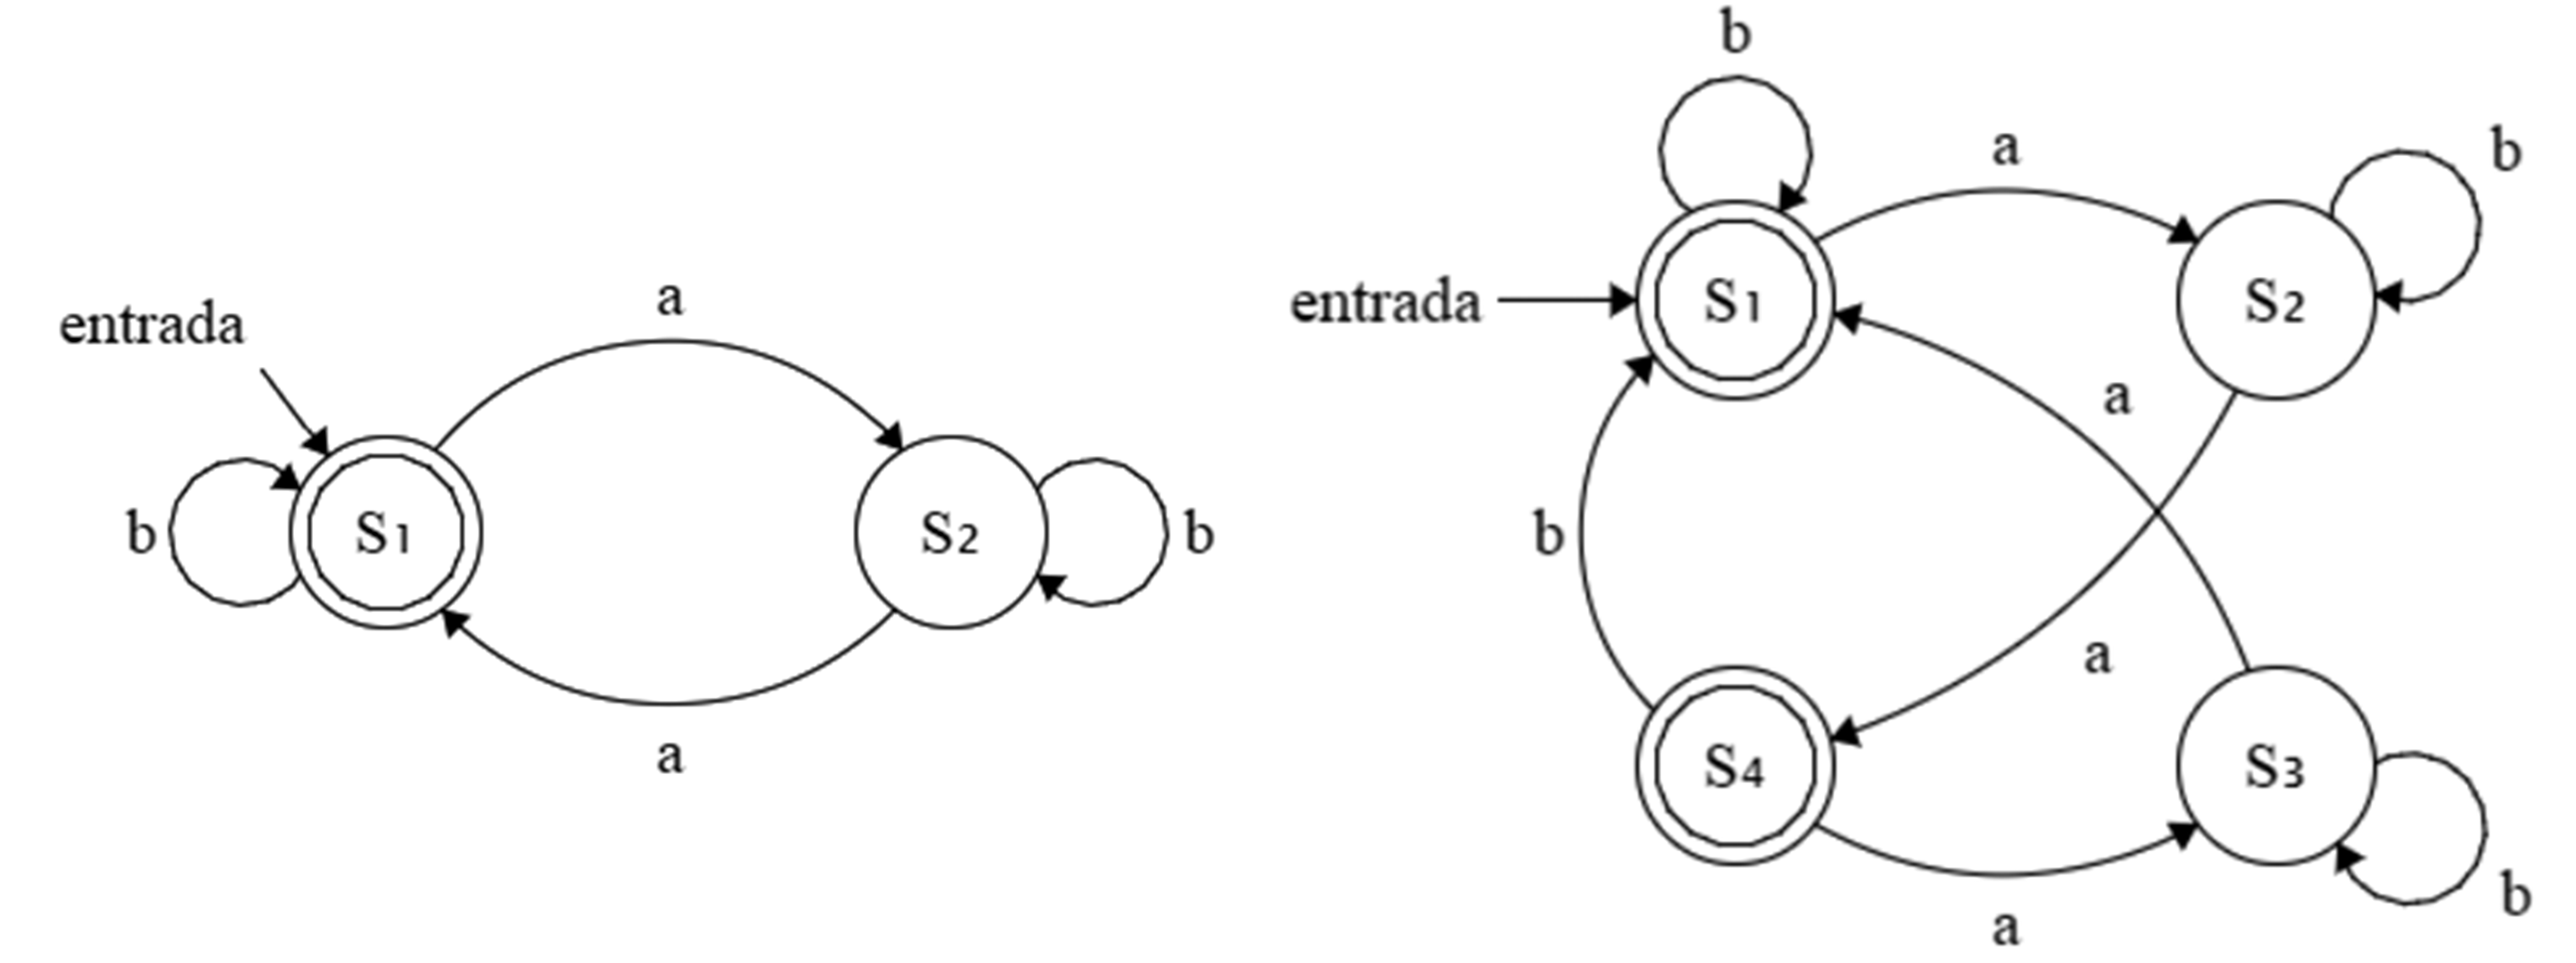
\includegraphics[width=0.75\linewidth]{exemplo.png}
  \caption{Autômato $M_1$ a esquerda e Autômato $M_2$ a direita.}
  \label{fig:exemplo}
\end{figure}

Apesar de $M_2$ ser visivelmente maior e mais complexo que $M_1$, o autômato $M_2$ reconhece a mesma linguagem que o autômato $M_1$ da Figura~\ref{fig:exemplo}. É possível demonstrar que, para cada linguagem regular, existem infinitos autômatos que a reconhecem. Como decidir então se o autômato-resposta dado por um aluno reconhece a linguagem pedida? No caso do sistema que iremos desenvolver isso se reduz ao seguinte problema:
  
\noindent\textbf{Problema:} Decidir se dois autômatos finitos determinísticos reconhecem a mesma linguagem.

\section{\textsc{Objetivos e Metodologia}}

Estudar e implementar o algoritmo de Moore (MOORE, 1956) para minimização e equivalência de AFDs.

Estudar e implementar o algoritmo de Hopcroft e Karp (HOPCROFT; KARP, 1971) para testar a equivalência de AFDs; 

Desenvolvimento do sistema de apoio a aprendizagem da disciplina Linguagens Formais e Autômatos

Reuniões semanais com o orientador, afim de acompanhar o progresso do desenvolvimento do sistema e esclarecer eventuais dúvidas.


\section{\textsc{Resultados}}


\begin{figure}
  \centering
  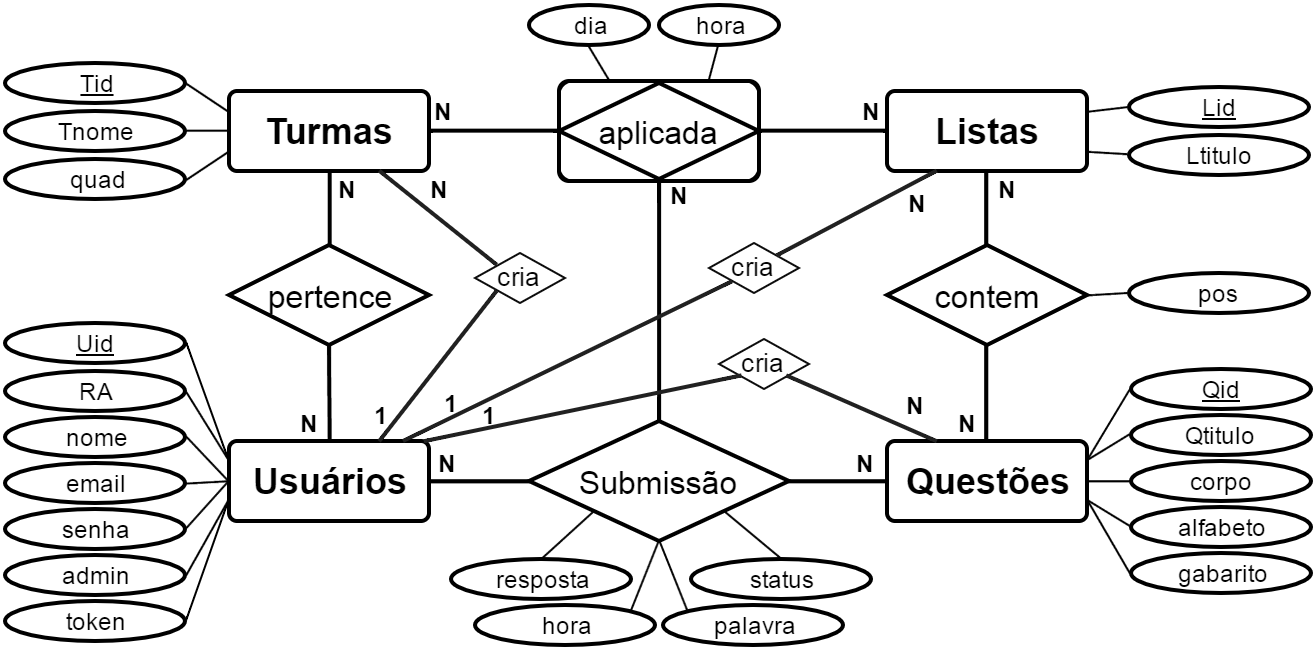
\includegraphics[width=0.9\linewidth]{diagDER.png}
  \caption{Diagrama de Entidade e Relacionamento do DFAjudge}
  \label{fig:DER}
\end{figure}


\textit{Tipos de Feedback}

Teste com a Turma de LFA 2016q2


\section{\textsc{Discussão}}



\section{\textsc{Conclusão}}




\section{\textsc{Referências}}
%// apenas citados neste poster

HOPCROFT, J. E.; MOTWANI, R.; ULLMAN, J. D. \textit{Automata theory, languages, and computation}. International Edition, v. 24, 2006.

MOORE, Edward F. \textit{Gedanken-experiments on sequential machines}. Automata studies, v. 34, p. 129-153, 1956.

HOPCROFT, John E.; KARP, Richard M. \textit{A Linear Algorithm for Testing Equivalence of Finite Automata}. Technical report of Cornell University, p. 71–114, 1971.

\section{\textsc{Agradecimentos}}
Este trabalho foi financiado pelo Programa de Iniciação Científica da UFABC.
%%%%%Deve conter agradecimento agência de fomento
%\vspace{1cm}
%\noindent\textbf{Este trabalho foi financiado pelo Programa de Iniciação Científica da UFABC. }


\end{multicols}
\end{document}